\documentclass[preprint]{elsarticle}
\usepackage{graphicx}
\graphicspath{ {D:/semesters/sem6/btp/} }
\begin{document}
\section{Estimation of Firewall Security Coefficient}

The Firewall is the core of a well-defined network security policy. The goal of the Check Point Firewall Rule Base is to create rules that only allow the specified connections.
\subsection{Order of Rule Enforcement}
The Firewall inspects connections and enforces the Rule Base in a sequential manner. The Firewall inspects each connection that comes to the network and compares the data (source, destination, service, etc.) to the first rule. If the connection matches the rule, the Firewall applies the action of that rule. If the connection does not match the rule, the Firewall continues with the next rule in the Rule Base. \\

\end{subsection} \\


 \begin{figure}[h]
 \centering
 \begin{minipage}{.5\columnwidth}
  \centering
  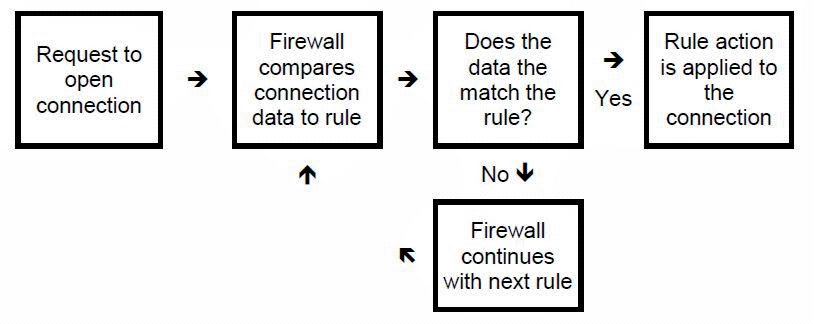
\includegraphics[width=1\columnwidth, clip=true]{1.png}
  \end{minipage}
 \end{figure}

\subsection{Firewall rule priority}
Because you can make firewall rules that have apparent conflicts, it is important to understand the order in which the rules are processed:
\subsection{Authenticated bypass}
These are rules in which the Override block rules option is selected.     These rules allow   matching network traffic that would otherwise be blocked. The network traffic must be authenticated by using a separate connection security rule. You can use these rules to permit access to the computer to authorized network administrators and authorized network troubleshooting devices.
\end{subsection}
\subsection{Block connection}
       These rules block all matching inbound network traffic.
\end{subsection}
\subsection{Allow connection}
        These rules allow matching inbound network traffic. Because the default  behavior is to block unsolicited inbound network traffic, you must create an allow rule to support any network program or service that must be able to accept inbound connections.\\
      The coefficient of firewall security m should depend on the types of files(data) under consideration,defined firewall security rules in the firewall rule base and the reliability and efficiency of the firewall. We propose a method for
          quantifying the coefficient m of firewall security as: \\
          $$m=-{\log_e (p+q-pq)}$$      \\
          where q quantifies the response of the files to the defined security rules.
For our work we can add certain rules by monitoring the behavior of attacker class.when the files will be received in targetted class they will be checked according to the rules defined in the firewall rule base.If they response correctly to all these rules then q=0 and if they don't match any of the rules then q=1 and it is assumed that the malware propagation rate can be reduced by p fraction when all received files follow the defined security rules.

\end{subsection}
\end{subsection}

\end{section}
\end{document} 